% -----------------------------------------------
% Template for ISMIR Papers
% 2015 version, based on previous ISMIR templates
% -----------------------------------------------

\documentclass{article}
\usepackage{ismir,amsmath,cite}
\usepackage{graphicx}
\usepackage{color}
\usepackage{booktabs}
\usepackage{microtype}
\usepackage{units}
\usepackage{paralist}
% Title.
% ------
\title{Chord Detection Using Deep Learning}

\DeclareMathOperator*{\pool}{pool}
\DeclareMathOperator*{\sigm}{sigm}
\DeclareMathOperator*{\softmax}{softmax}

% Single address
% To use with only one author or several with the same address
% ---------------
%\oneauthor
% {Names should be omitted for double-blind reviewing}
% {Affiliations should be omitted for double-blind reviewing}

% Two addresses
% --------------
%\twoauthors
%  {First author} {School \\ Department}
%  {Second author} {Company \\ Address}

% Three addresses
% --------------
\twoauthors
  {Xinquan Zhou} {Center for Music Technology \\ Georgia Institute of Technology\\  {\tt\small royzxq@gmail.com}}
  {Alexander Lerch} {Center for Music Technology \\ Georgia Institute of Technology\\ {\tt\small alexander.lerch@gatech.edu}}
  %{Third author} {Affiliation3 \\ {\tt author3@ismir.edu}}/

% Four addresses
% --------------
%\fourauthors
%  {First author} {Affiliation1 \\ {\tt author1@ismir.edu}}
%  {Second author}{Affiliation2 \\ {\tt author2@ismir.edu}}
%  {Third author} {Affiliation3 \\ {\tt author3@ismir.edu}}
%  {Fourth author} {Affiliation4 \\ {\tt author4@ismir.edu}}

\begin{document}
%
\maketitle
%
\begin{abstract}
In this paper, we utilize deep learning to learn high-level features for audio chord detection. The learned features, obtained by a deep network in bottleneck architecture, give promising results and outperform state-of-the-art systems. We present and evaluate the results for various methods and configurations, including input pre-processing, a bottleneck architecture, and SVMs vs.\ HMMs for chord classification. 
\end{abstract}
%
\section{Introduction}
The goal of automatic chord detection is the automatic recognition of the chord progression in a music recording. It is an important task in the analysis of western music and music transcription in general, and it can contribute to applications such as key detection, structural segmentation, music similarity measures, and other semantic analysis tasks. Despite early successes in chord detection by using pitch chroma features \cite{fujishima1999realtime} and Hidden Markov Models (HMMs) \cite{sheh2003chord}, recent attempts at further increasing the detection accuracy are only met with moderate success \cite{ueda2010hmm,cho2013mirex}.

In recent years, deep learning approaches have gained significant interest in the machine learning community as a way of building hierarchical representations from large amounts of data. Deep learning has been applied successfully in various fields; for instance, a system for speech recognition utilizing deep learning was able to outperform state-of-the-art systems not using deep learning \cite{hinton2012deep}. Several studies indicate that deep learning methods can be very successful when applied to Music Information Retrieval (MIR) tasks, especially when used for feature learning \cite{lee2009unsupervised,battenberg2012analyzing,humphrey2012moving,hamel2010learning}. Deep learning, with its potential to untangle complicated patterns in a large amount of data, should be well suited for the task of chord detection.

In this work, we investigate Deep Networks (DNs) for learning high-level and more representative features in the context of chord detection, effectively replacing the widely used pitch chroma intermediate representation. 
We present individual results for different pre-processing options such as time splicing and filtering (see Sect.~\ref{sec:pre-proc}), architectures (see Sect.~\ref{sec:arch}), and output classifiers (see Sect.~\ref{sec:class}). %Since chords last for a period of time instead of static and instantaneous, we apply time splicing and convolution to account for relations between nearby frames. Then we can derive transition probability between chords from our training set and use the high-level probabilistic features as emission probability to decode the whole chord sequence. Alternatively we also train SVMs with same features and do the static classification frame by frame.

%The definition of chords is, simply speaking, \"simultaneous sounding of two or notes". But in reality this is not the case. Real music often generate not only chord tones but nonchord tones with no guarantee of simultaneity. To make it more complicated, sometimes either some notes are missing or more notes are added-on into a chord. Thus, traditional chord detection systems exhibit a set of practical difficulties. Deep learning has a great potential in entangling complicated patterns within large data. Therefore, although chord detection is one of the most difficult and challenging tasks for music analysis, applying deep learning methods is much potentially promising. 
%

%\begin{figure}
% \centerline{\framebox{
% 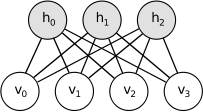
\includegraphics[width=\columnwidth]{rbm.png}}}
% \caption{DBN with one visible layer and one hidden layer}
% %\label{fig:example}
%\end{figure}

\section{related work}
During the past decade, deep learning has been considered by the machine learning community to be one of the most interesting and intriguing research topics. Deep architectures promise to remove the necessity of custom-designed and manually selected features as neural networks should be more powerful in disentangling interacting factors and thus be able to create meaningful high-level representations of the input data. Generally speaking, deep learning combines deep neural networks with an unsupervised learning model. Two major learning models are widely used for unsupervised learning: Restricted Boltzmann Machines (RBMs) \cite{hinton2006fast}  and Sparse Auto Encoders \cite{poultney2006efficient}. A deep architecture comprises multiple stacked layers based on one of these two models. These layers can be trained one by one, a process that is referred to as ``pre-training'' the network. In this work, we employ RBMs to pre-train the deep architecture in an unsupervised fashion; this is called a Deep Belief Network (DBN) \cite{hinton2006fast}. DBNs, composed of a stack of RBMs, essentially share the same topology with general neural networks: DBNs are generative probabilistic models with one visible layer and several hidden layers. 

Since Hinton et al.\ proposed a fast learning algorithm for DBNs \cite{hinton2006fast}, it has been widely used for initializing deep neural networks. In deep structures, each layer learns relationships between units in lower layers. The complexity of the system increases with an increasing number of RBM layers, making the structure~---in theory---~more powerful. An extra softmax output layer can be added to the top of the network (see \eqnref{softmax}) \cite{martinetz1993neural}; its output can be interpreted as the likelihood of each class.

LeCun and Bengio introduced the idea of applying Convolutional Neural Networks (CNNs) to images, speech, and other time-series signals \cite{lecun1995convolutional}. This approach allows to deal with the variability in time and space to a certain degree, as CNNs can be seen as a special type of neural network in which the weights are shared across the input within a certain spatial or temporal area. The weights thus act as a kernel filter applied to the input. CNNs have been particularly successful in image analysis. For example, Norouzi et al.\ used Convolutional RBMs to learn shift-invariant features \cite{norouzi2009stacks}. 
%\begin{figure}
% \centerline{\framebox{
% 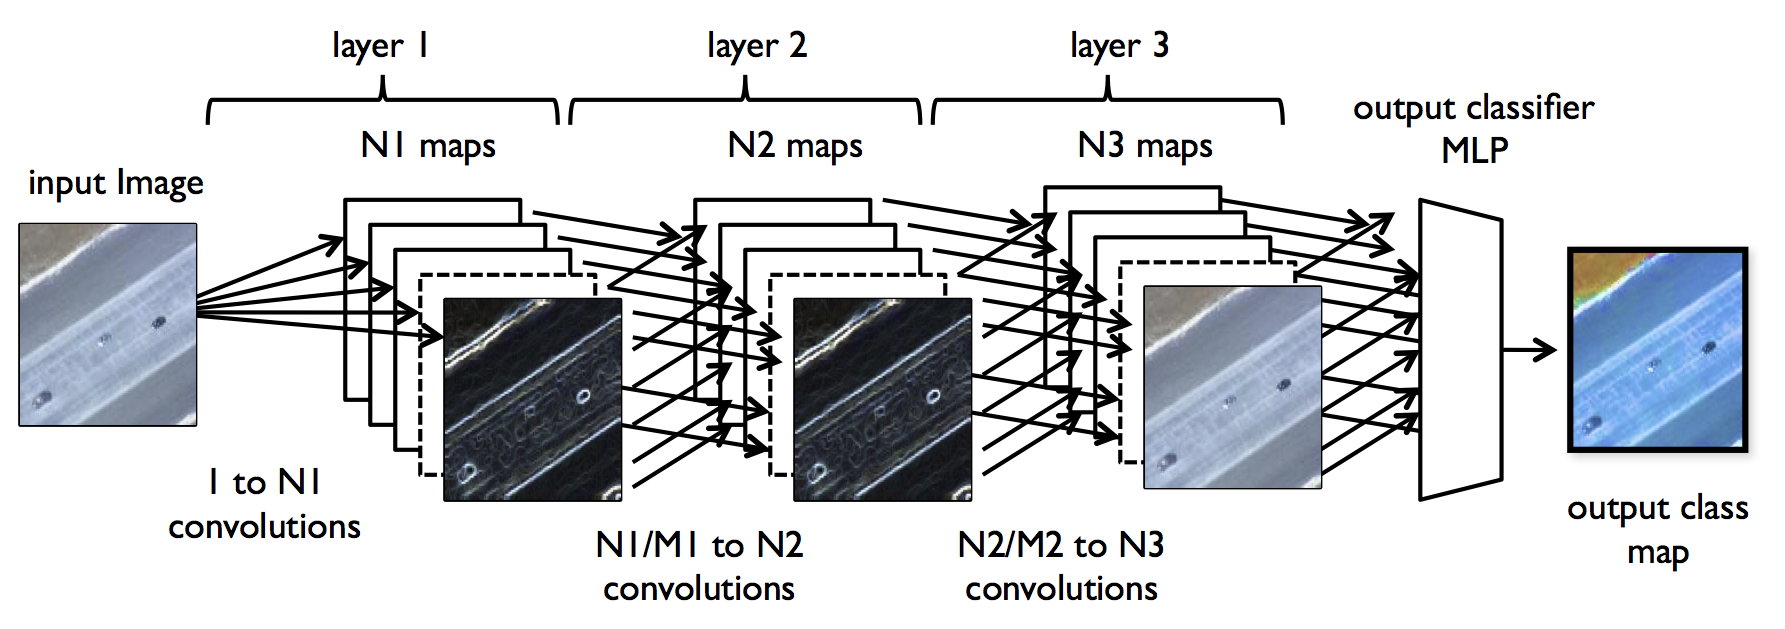
\includegraphics[width=\columnwidth]{neuralnet.png}}}
% \caption{CNNs used for image classification}
% \label{fig:cnn}
%\end{figure}

The results of a network depend largely on the network architecture. For example, Grezl et al.\ used a so-called bottleneck architecture neural network to obtain features for speech recognition and showed that these features improve the accuracy of the task \cite{grezl2007probabilistic}. The principle behind the bottleneck-shaped architecture is that the number of neurons in the middle layer is lower than in the other layers as shown in Fig.~\ref{fig:bottleneck}. A network with bottleneck can be structured in two sections:  
\begin{inparaenum}[(i)]
    \item   Section~1 from the first layer to the bottleneck layer, with a gradual decrease of the number of neurons per layer, functions as an encoding or compression process which compacts relevant information and discards redundant information, and 
    \item   Section~2 from the bottleneck layer to the last layer with a gradual increase in the number of neurons per layer. The function of this part can be interpreted as a decoding process. An additional benefit of bottleneck architectures is that they can reduce overfitting by decreasing the system complexity.
\end{inparaenum}

Recently, more researchers investigated deep learning in the context of MIR. Lee et al.\ pioneered the application of convolutional deep learning for audio feature learning \cite{lee2009unsupervised}. Hamel et al.\ used the features learned from music with a DBN for both music genre classification and music auto-tagging \cite{hamel2010learning}; their system was successful in MIREX 2011 with top-ranked results. Battenberg employed a conditional DBN to analyze drum patterns \cite{battenberg2012analyzing}. The use of deep architectures for chord detections, however, has not yet been explored, although modern neural networks have been employed in this field. For instance, Boulanger et al.\ investigated recurrent neural networks \cite{boulanger2013audio} and Humphrey has explored CNNs \cite{humphrey2012rethinking,humphrey2012learning}. While they also used the concept of pre-training, their architectures have only two or 3 layers and thus cannot be called ``deep''.
\begin{figure}
 \centerline{\framebox{
 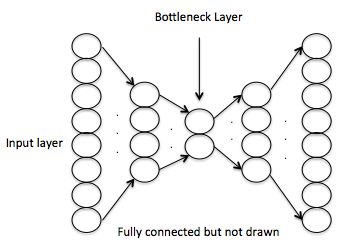
\includegraphics[scale=0.55]{bottleneck}}}
 \caption{Visualization of a bottleneck architecture}
 \label{fig:bottleneck}
\end{figure}

The basic buildings blocks of most modern approaches to chord detection can be traced back to two seminal publications: Fujishima introduced pitch chroma vectors extracted from the audio as input feature for chord detection \cite{fujishima1999realtime} and Sheh et al.\ proposed to use HMMs for representing chords as hidden states and to model the transition probability of chords \cite{sheh2003chord}. Since then, there have been a lot of studies using chroma features and HMMs for chord detection\cite{papadopoulos2007large,cho2010exploring}. Examples for recent systems are  Ni et al., using a genre-independent chord estimation method based on HMM and chroma features \cite{ni2012using} and Cho and Bello, who used multi-band features and a multi-stream HMM for chord recognition \cite{cho2013mirex}. Training HMMs with pitch chroma features arguably is the standard approach for this task and the progress is less marked by major innovations but by optimizing and tuning specific components. 

%In this work, we employ deep learning to come up with a novel system for chord detection. 

%\begin{figure}
% \centerline{\framebox{
% \includegraphics[width=\columnwidth]{1.png}}}
% \caption{Underlying chord states from melody}
% %\label{fig:example}
%\end{figure}

\section{System Overview}
Figure~\ref{fig:overview} gives an overview of all components and processing steps of the presented system. The following section will discuss all of these steps in detail.
\begin{figure}
 \centerline{\framebox{
 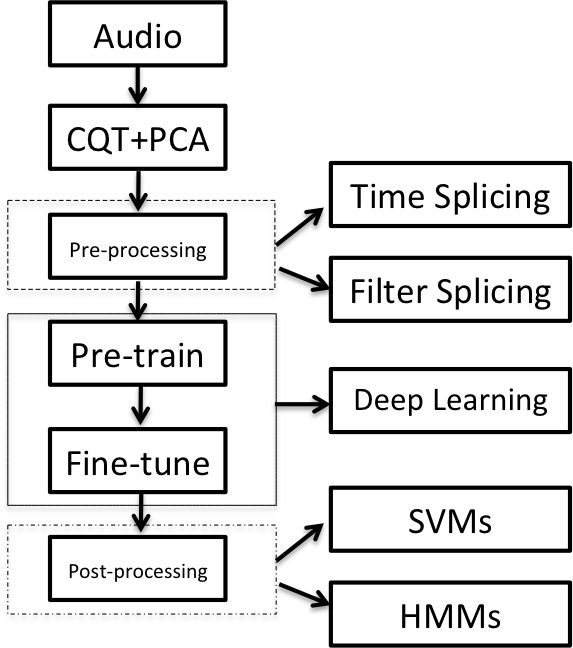
\includegraphics[scale=0.7]{flowchart.png}}}
 \caption{The overview of our system}
 \label{fig:overview}
\end{figure}

\subsection{Input Representation}\label{sec:input}
The input audio is converted to a sample rate of \unit[11.025]{kHz}. Then, a Constant Q transform (CQT) is applied. 
The CQT \cite{brown1991calculation} is a perceptually inspired time-frequency transformation for audio. The resulting frequency bins are equally spaced on a logarithmic (``pitch'') scale. It has the advantage of providing a more musically and perceptually meaningful spectral representation than the DFT. 
We used an implementation of the CQT as a filterbank of Gabor filters, spaced at \unit[36]{bins per octave}, i.e., \unit[3]{bins per semitone}, yielding \unit[180]{bins} representing a frequency range spanning from \unit[110]{Hz} to \unit[3.520]{kHz}. Finally, we used Principal Component Analysis (PCA) for decorrelation, and applied Z-Score normalization\cite{sola1997importance}. 

\subsection{Pre-processing}\label{sec:pre-proc}
Neighboring frames of the input representation can be expected to contain similar content, as chords will not change on a frame-by-frame basis. In order to take into account the relationship between the current frame and previous and future frames, we investigate the application of several pre-processing approaches.

\subsubsection{Time Splicing}
Time splicing is a simple way to extend the current frame with the data of neighboring frames by concatenating the frames into one larger superframe. In first order time splicing, we concatenate the current frame, the previous frame, and the following frame. Thus, each superframe consists of three neighboring frames. Since the same operation will be applied to all frames, there will be overlap introduced between neighboring superframes. %We conduct such operation along over all frames in each piece with different splice amount. 
%\begin{figure}
% \centerline{\framebox{
% 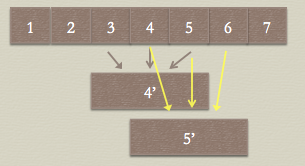
\includegraphics[width=\columnwidth]{timesplice}}}
% \caption{Illustration for time splicing}
% \label{fig:splicing}
%\end{figure}

\subsubsection{Convolution}
CNNs are extensively used in tasks with highly correlated inputs (e.g., the recognition of hand-written digits). Many time series show similar properties so that CNNs seem to be an appropriate choice in the context of audio, too. Essentially, CNNs have one or more convolutional layers between the input and lower layers of the neural network. The function of a convolutional layer can be interpreted as the application of a linear filter plus a non-linear transformation, sometimes also combined with a pooling operation:
\begin{equation}\label{Covulution}
Y = \pool(\sigm(K \ast X + B)),  
\end{equation}
in which $Y$ is the output of a convolutional layer, $K$ is the linear kernel filter (i.e., the impulse response), $X$ is the input, $B$ is the bias, $\sigm()$ is a non-linear transform, and $\pool()$ is a down-sampling operation. The uniqueness of convolutional networks stems from the convolution operation applied to the input $X$. Since, unfortunately, we had no access to a deep learning toolbox with support for the convolution operation in the time domain, we opted to employ an optional pre-processing step inspired by CNNs, namely by applying filters to the input of the network. However, instead of learning the filters, we evaluate several manually designed filters: a single-pole low pass filter and two FIR low pass filters with exponentially shaped impulse responses.
%Instead of training the filters automatically, we can make use of the prior knowledge to design the filters manually. In the case of chord detection, given we mainly want to extract time information by convolution, so we design time domain filters. \\
%A simple choice is low pass filter family. 
The single pole low pass filter produces the output $y$ for an input $x$, given the parameter $\alpha$:
\begin{equation}\label{IIR}
y_{n} = (1-\alpha) y_{n-1} + \alpha x_{n}
\end{equation}
We apply anti-causal filtering and filter the signal in both directions so that the resulting overall filter has a zero-phase response.

%Under the assumption that the frame that is located in the middle of a chord is way more obvious and easier to be detected than the frame that is located at the boundary of a chord, w
The other two low pass filters have exponential decay shaped impulse response. The difference equations are given in \eqnref{filter1} and \eqnref{filter2}. 
\begin{equation}\label{filter1}
y_{1}(n) = \sum_{k=1}^N a^{-k+1} x(n-N+k)
\end{equation}
\begin{equation}\label{filter2}
y_{2}(n) = \sum_{k=1}^N a^{-k+1} x(n+N-k)
\end{equation} 
The filter length is $N$ and $a$ is the exponential base. 
These two filters are not centered around the current frame anymore but shifted by $N$ frames. Their impulse responses are symmetric to each other. One could interpret these filters as focusing on past and future frames, respectively. The presented filters will be referred to as ``extension filters". 

The ideas of splicing and convolution can be combined, as exemplified in Fig.~\ref{fig:filtersplice}.
%In a further processing, we combine the ideas of time splicing and convolution: we either conduct time splicing on the output of the low pass filter, or splice the output of different filters together, as in figure 4.
\begin{figure}
 \centerline{\framebox{
 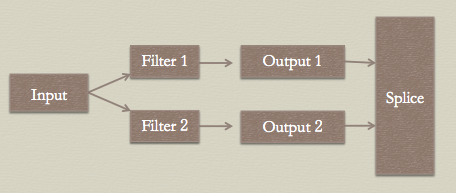
\includegraphics[scale=0.6]{CNN}}}
 \caption{Splicing output of different filters}
 \label{fig:filtersplice}
\end{figure}

Furthermore, similar to the process in CNNs, a maximum pooling operation on the output of the spliced filters is optionally applied. The operation takes the maximum value among different filters per ``bin". 
 
\subsection{Training}\label{sec:train}
It is impractical to train DNNs directly with back propagation using gradient decent due to their deep structure and the limited amount of training samples. Therefore, the network is usually initialized by an unsupervised pre-training step. As our network consists of RBMs, Gibbs sampling can be used for training \cite{hinton2006fast}. The objective is to retain as much information as possible between input and output. 

The computation for layer $l$ can be represented as:
\begin{equation}\label{dbn}
Y_{l} = \sigm(W_{l}X_{l} + B_{l}) ,
\end{equation}  
which is identical to many traditional neural networks. Thus, a standard back propagation can be applied after pre-training to fine-tune the network in a supervised manner. The loss criterion we use in this work is cross-entropy.  

\subsection{Architecture}\label{sec:arch}
We investigate a deep network with $6$ layers in two different architectures. The common architecture features the same amount of neurons in every layer, in our case $1024$. The bottleneck architecture has $256$ neurons in the middle layer and $512$ neurons in the layers neighboring the middle layer. The remaining layers consist $1024$ neurons each (compare \cite{grezl2007probabilistic}).
A softmax output layer is stacked on top of both architectures as described by \eqnref{softmax}.
\begin{equation}\label{softmax}
\softmax(Y_{l}) = \frac{\exp(Y_{l})}{\sum_{k=1}^N \exp(Y_{k})}
\end{equation}
The network is implemented using the Kaldi package developed by John Hopkins University \cite{povey2011kaldi}.
 
\section{Classification}\label{sec:class}
The output of the softmax layer can be interpreted as the likelihood of each chord class; simply taking the maximum will provide a class decision (this method will be referred to as \textit{Argmax}). Alternatively, the output can be treated as intermediate feature vector that can be used as an input to other classifiers for computing the final decision. 
\subsection{Support Vector Machine}
Support Vector Machines (SVMs) are, as widely used classifiers with generally good performance. The SVM is trained using the output of the network as features, and the classification is carried out frame by frame. The classification is followed by a simple prediction smoothing.
\subsection{Hidden Markov Model}
HMMs are, as pointed out above, the standard classifier for automatic chord detection because the characteristics of the task fit the HMM approach well: Chords are hidden states that can be estimated from observations (feature vectors extracted from the audio signal), and the likelihood of chord transitions can be modeled with transition probabilities. 
Modified HMMs such as ergodic HMMs and key-independent HMMs have been also explored for this task \cite{papadopoulos2007large,lee2008acoustic}. In this work we are mostly interested in the performance comparison between high-level features, so a simple first-order HMM is used. 
Given the probabilistic characteristic of the softmax output layer, it can be directly as emission probabilities for the HMM. Therefore, there is no need to train the HMM using, e.g., the commonly used Baum-Welch algorithm. Instead, the histogram of each class in our training is used as initial probabilities, and the bigram of chord transitions is used to compute the transition probabilities. Finally, we employ the Viterbi decoding algorithm to find the globally optimal chord sequence. 

\section{Evaluation procedure}
\subsection{Dataset}
Our dataset is a combination of several different datasets, yielding a 317-piece collection. The data is composed of 
\begin{compactitem}
	\item   $180$ songs from the \textit{Beatles dataset} \cite{mauch2009omras2},
    \item   $100$ songs from the \textit{RWC Pop dataset} \cite{goto2002rwc}, 
    \item   $18$ songs from the \textit{Zweieck dataset} \cite{mauch2009omras2}, and 
    \item   $19$ songs from \textit{Queen dataset} \cite{mauch2009omras2}.
\end{compactitem}  
The pre-processing as described in Sect.~\ref{sec:pre-proc} ensures identical input audio formats.

\subsection{Methodology}

The dataset is divided randomly into two parts: 80\% for the training set and 20\% for the test set. On the training scale, we use a frame-based strategy, which means we divide each song into frames, and treat each frame as an independent training sample. On average each song is divided into about 1200 frames resulting in approximately 300k training samples and approximately 76k test samples. 

Within the training set, 10\% of the data is used as a validation set. For the post-processing, all data in the training set will be used to train the post-classifier.

Time constraints and the workload requirements for training deep networks made a cross validation for evaluation impractical. 

The chosen ground truth for classification are major and minor triads for every root note, resulting in a dictionary of $24+1$ chord labels.
Ground truth time-aligned chord symbols are mapped to this major/minor dictionary:
\begin{equation}
Chord_{majmin} \subset \{N\} \cup \{S \times {maj,min}\}
\end{equation}
with $S$ representing the 12 pitch classes (root notes) and $N$ being the label for unknown chords. In the calculation of the detection accuracy, the following chord types are mapped to the corresponding major/minor in the dictionary: triad major/minor and seventh major/minor. Other chord types are treated as unknown chords. For instance, G:maj and G:maj7 are mapped to `G:maj'; G:dim and G:6 are all mapped to `N'. The histogram of chords in our dataset after such mapping is shown in Fig.~\ref{fig:distrib}. 
\begin{figure}
 \centerline{\framebox{
 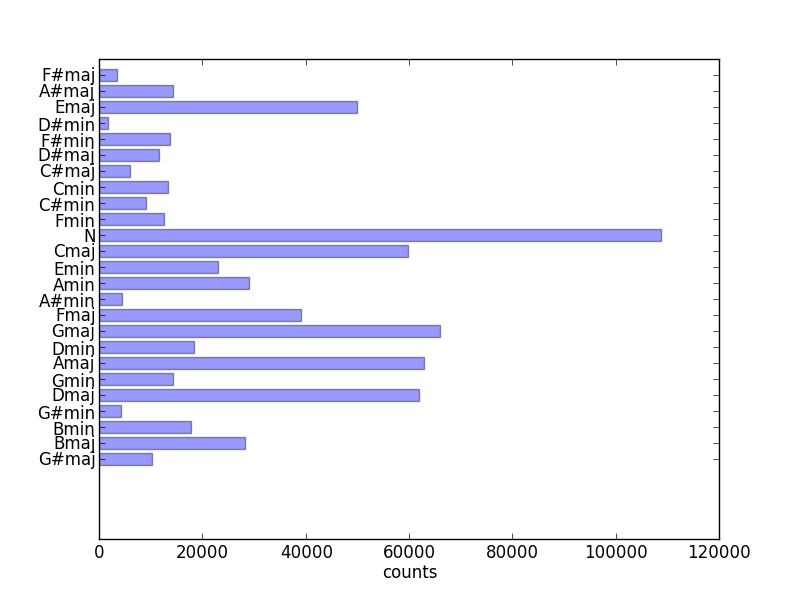
\includegraphics[width=\columnwidth]{chordDistrib}}}
 \caption{Chords histogram}
 \label{fig:distrib}
\end{figure}

\subsection{Evaluation Metric}
The used evaluation metric is the same as proposed in the audio chord detection task for MIREX 2013: the Weighted Chord Symbol Recall (WCSR). WCSR is defined as the total duration of segments with correct prediction as formulated in \eqnref{csr}:   
\begin{equation}\label{csr}
WCSR = \frac{1}{N} \sum_{k=1}^n C_{k},
\end{equation}
in which $n$ is the number of test samples (songs), $N$ is the total number of frames in all test samples, and $C_{k}$ is the number of frames that are correctly detected in the $k$th sample. 

\section{Experiments}

\subsection{Post-classifiers}
In this experiment, the network is initialized with pre-training, followed by fine tuning using back propagation. This configuration will be referred to as $DN_{DBN-DNN}$.
No pre-processing is applied to the data; the input is simply the input representation (CQT followed by PCA) as described in Sect.~\ref{sec:input}. The chosen architecture is the bottleneck architecture. 
Three different classifiers are compared: the maximum of the softmax output (Argmax), an SVM, and an HMM. 
\begin{table}
\centering
\begin{tabular*}{\columnwidth}{@{\extracolsep{\fill}}llr}
%\begin{tabular}{@{}llr@{}}
\toprule
\textbf{Training Scenario} & \textbf{Classifier} & \textbf{WCSR}  \\ \hline

$DN_\mathrm{DBN-DNN}$         & Argmax()            & 0.648 \\ 
$DN_\mathrm{DBN-DNN}$          & SVM            & 0.645 \\ 
$DN_\mathrm{DBN-DNN}$         &  HMM           & \textbf{0.755} \\ \bottomrule
\end{tabular*}
\caption{Chord detection performance using different post-classifiers}
\label{tab:dbn-dnn}
\end{table}

The results listed in Table~\ref{tab:dbn-dnn} are unambiguous and unsurprising: the HMM with Viterbi decoding outperforms the SVM; using HMMs with a model for transition probabilities is an appropriate approach to chord detection as it models the dynamic properties of chord progressions, which cannot be done with non-dynamic classifiers such as SVMs. One noteworthy result is that the SVM does not improve the WCSR compared to the direct (Argmax) output of the network. Apparently, the SVM is not able to improve separability of the learned output features.
\subsection{Pre-processing}
As stated in Sect.~\ref{sec:pre-proc}, we are interested in the application of different filters in the pre-processing stage. 
In the first experiment (\textit{Filtering}), an anti-causal single pole filter (see \eqnref{IIR}) is evaluated with the parameter $\alpha$ set to $0.25$, $0.5$, and $0.75$, respectively. The second experiment (\textit{Spliced Filters}), splices these filter outputs with the outputs of the extension filters as introduced in Sect.~\ref{sec:pre-proc}. These experiments are carried out with the  $DN_\mathrm{DBN-DNN}$ training scenario, a bottleneck architecture, and an HMM classifier. Table~\ref{table:filter} lists the results of these pre-processing variants.
%\begin{figure}
% \centerline{\framebox{
% 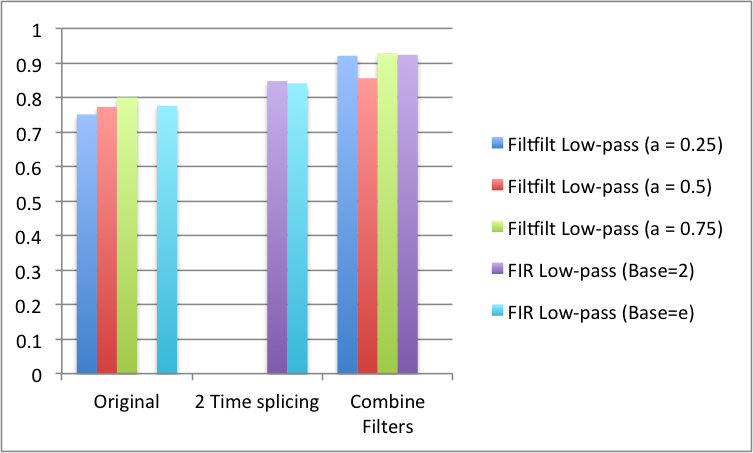
\includegraphics[width=\columnwidth]{filters.png}}}
% \caption{Comparison between different filters}
% \label{tab:filter}
%\end{figure}
\begin{table}[t]
\begin{tabular*}{\columnwidth}{@{\extracolsep{\fill}}llr}
\toprule
$\alpha$    & Pre-processing  & WCSR  \\  \midrule
0.25 & Filtering             & 0.758 \\
0.25 & Spliced Filters & 0.912 \\
0.5  & Filtering             & 0.787 \\
0.5  & Spliced Filters & 0.857 \\
0.75 & Filtering             & 0.798 \\
0.75 & Spliced Filters & \bf{0.919} \\ \bottomrule
\end{tabular*}
\caption{Chord detection performance using different filter parameters}


\label{table:filter}

\end{table}
It can be observed that the network trained with filtered inputs slightly outperforms the network without pre-processing; splicing the filtered input with the extension filter outputs increases the results drastically. 


\subsection{Architecture}
\subsubsection{Common vs.\ Bottleneck}
The results of Grezl et al.\ indicate that a bottleneck architecture should be more suitable to learn high-level features than a common architecture and reduce overfitting \cite{grezl2007probabilistic}. In order to verify these characteristics for our task, the performance of both architectures is evaluated in comparison. The results are listed in Table~\ref{tab:arch} for three pre-processing scenarios: no additional pre-processing (\textit{None}), \textit{Spliced Filters} and spliced filters followed by a max pooling (\textit{Pooling}). In order to allow conclusions about overfitting, both the WCSR of the test set and the training set are reported.
All results are computed for the $DN_\mathrm{DBN-DNN}$ training scenario with HMM classifiers.

\begin{table}
\centering
\begin{tabular*}{\columnwidth}{@{\extracolsep{\fill}}llcr}
\toprule
\textbf{Architecture}                   & \textbf{Pre-processing}                      & \begin{tabular}[c]{@{}c@{}}\textbf{Training}\\ \textbf{WCSR}\end{tabular} & \textbf{WCSR}  \\ \midrule
Common                         & None                                & 0.843                                                      & 0.703 \\
Bottleneck                     & None                                & 0.855                                                      & 0.755 \\
%Common                         & 2 Time Splicing                     & 0.903                                                  & 0.712 \\
%\multicolumn{1}{l}{Bottleneck} & \multicolumn{1}{l}{2 Time Splicing} & 0.892                                 & 0.821 \\ 
Common     & Spliced Filters & \textbf{0.985} & 0.876 \\
Bottleneck & Spliced Filters & 0.936 & \textbf{0.919} \\ 
Common & Pooling & 0.965 & 0.875 \\ 
Bottleneck & Pooling & 0.960 & 0.916 \\ \bottomrule
\end{tabular*}
\caption{Chord detection performance for different architectures and pre-processing steps}
\label{tab:arch}
\end{table}

The results show that the bottleneck architecture gives significantly better results ($p=0.023$) on the test set (\textit{WSCR}). Note that this is not true for the training set (\textit{Training WSCR}), for which the common architecture achieves results in the same range or better than the bottleneck architecture. The difference between the results on the training set and the test set are thus much larger for the common architecture than for the bottleneck architecture.
The bottleneck architecture is clearly advantageous to use in this task: it reduces complexity and thus the training workload and increases the classification performance significantly. Furthermore, the comparison of classifier performance between training and test set in Table~\ref{tab:arch} clearly indicates that the common architecture tends to fit more to the training data, and is thus more prone to overfitting. 


\subsubsection{Single-Label vs.\ Multi-Label}
As mentioned above, the pitch chroma is the standard feature representation for audio chord detection. Since we use the output of our deep network as feature, it seems an intuitive choice to learn pitch class information (and thus, a pitch chroma) instead of the chord classes. By doing so, the number of outputs is reduced by a factor of two (or higher in the case of more chords), and there would also be a closer relation between the output and the input representation, the CQT. Therefore, the abstraction and complexity of the task might be decreased. It will, however, lead to another issue: the single-label output (one chord per output) will be changed into a multi-label output (multiple pitches per output). Therefore, the learning has to be modified to allow multiple simultaneous (pitch class) labels. 
The experiment is carried out with both Splicing and Filtering in the pre-processing, the $DN_\mathrm{DBN-DNN}$ training scenario, and HMM classifiers. Table~\ref{tab:multilabel} lists the results. 

\begin{table}
\centering
\begin{tabular*}{\columnwidth}{@{\extracolsep{\fill}}lr}
\toprule
\textbf{Learning Targets} & \textbf{WCSR}  \\ \midrule
Single-Label --- 25 Chord Classes & \textbf{0.919} \\
Multi-Label --- 12 Pitch Classes & 0.78  \\ \bottomrule
\end{tabular*}
\caption{Chord detection performance for single-label vs.\ multi-label learning}
\label{tab:multilabel}
\end{table}
Boulanger-Lewandowski et al.\ report combining chroma features with chord labels for their recurrent neural network and report a slightly improved result \cite{boulanger2013audio}. They do not, however, provide a detailed description of this combination. 
As can be seen from the table, the result for multi-label training is clearly lower than the result for single-label training.
Possible reasons for bad performance include
\begin{inparaenum}[(i)]
    \item   difficulties with multi-target learning, since it increases the difficulty to train; furthermore, our implementation of multi-label training might be sub-optimal as the same posterior is assigned to each target without any information on the pitch class energy, and
    \item   the issue that not all pitches always sound simultaneously in a chord (or might be missing altogether) might have larger impact on the multi-label training than on the single-label training.    
\end{inparaenum}


\subsection{Results \& Discussion}
It is challenging to compare the results to previously published results due to varying evaluation methodologies, metrics, and datasets. It seems that the results of Cho and Bello \cite{cho2013mirex}, who reported a performance of about 76\%, were computed with a comparable dataset. The recent MIREX results on Chord Detection generally show lower accuracy but use a different evaluation vocabulary. In order to provide a baseline result to put results into perspective, we present the results of Chordino \cite{mauch2010approximate} with the default settings, computed on our dataset. It should be pointed out that this comparison is unfair as Chordino is able to detect as many as 120 chords, compared to our 24. The label mapping strategies are another significant issue for Chordino. Our label mapping results in nearly sixth of the total label being ``N'', which might have negative impact on the Chordino results. The Chordino results are mapped to major/minor the same way as the ground truth annotations. The results are shown in Table~\ref{tab: final}. In the table, the \textit{Best Configuration} is using Bottleneck architecture, spliced filters $(\alpha = 0.75)$ as preprocessing, single label learning targets, and Viterbi decoding as post-classifier. The \textit{Best Configuration with Max Pooling} is the same as the best configuration except applying another max pooling layer after the spliced filters. The latter configuration has a much reduced computational workload. 
% Please add the following required packages to your document preamble:
% \usepackage{booktabs}
\begin{table}
\centering
\begin{tabular*}{\columnwidth}{@{\extracolsep{\fill}}lr}
\toprule
\textbf{Method}   &  \textbf{WCSR}   \\ \midrule
Chordino & 0.625       \\
Best Configuration &  0.919   \\ 
Best Configuration with Max Pooling & 0.916 \\ \bottomrule
\end{tabular*}
\caption{Comparison of the performance of the best configuration with Chordino}
\label{tab: final}
\end{table}
The presented results are clearly competitive with existing state-of-the-art systems.

%\subsection{Discussion}
%We presented a comprehensive system for chord detection, that is competitive with the existing start-of-the-art systems. Our DBN-DNNs model can learn a high-level probabilistic representations for chords. The Viterbi algorithm is applied to find a global optimal path based on the output of our DBN-DNNs as the predicted chord sequence. Furthermore, the bottleneck structure have a stronger learning ability for chords information than the common architecture. By the process of ``encoding" and ``decoding", the networks retain the ``essential information" but discard the redundant ones. The results also indicate that applying pre-processing will significantly increase the accuracy. That's because it will introduce temporal continuity and dynamics into feature representation. Intuitively, dynamic programming algorithms such as Viterbi decoding outperforms the static classifiers such as SVMs due to the dynamic property of chords. Therefore introducing transition probability makes more sense. 

\section{Conclusion \& Future Work}
In this work, we presented a system which applies deep learning to the MIR task of automatic chord detection. Our model is able to learn high-level probabilistic representations for chords across various configurations. We have shown that 
the use of a bottleneck architecture is advantageous as it reduces overfitting and increases classifier performance, and that
the choice of appropriate input filtering and splicing can significantly increase classifier performance.

Learning a pitch class vector instead of chord likelihood by incorporating multi-label learning proved to be less successful. The idea has, however, a certain appeal and would allow the number of output nodes to be independent of the number of chords to be detected. It is also conceivable to investigate a different option for the network output: instead of training chords or pitch classes we could~---~under the assumption that we are only after chords comprised of stacked third intervals~---~train the output with octave-independent third intervals in a multi-label scenario with $24$ output nodes.
%Combined with the appropriate pre-processing and post-processing, the performance can compete with state-of-the-art systems. Our pre-processing methods can retain temporal continuity and dynamics in our features; our post-processing could take care of the high-level musical context information. With a bottleneck structure, the overfitting issue s significantly reduced. With some practical limitations, multi-target training using pitch information does not work as well as single-target counterpart. The idea is, however, promising and worthy exploring in the future works. 

\bibliography{ISMIR2015template}
\end{document}
